\documentclass[12pt]{article}
\usepackage[fleqn]{amsmath}
\usepackage{amssymb}
\usepackage{amsthm}
\usepackage{amssymb}
\usepackage{tikz}
\usepackage{tipa}
\usepackage{pgfplots}
\pgfplotsset{width=10cm,compat=1.9}
\usepackage{hyperref}
\usepackage{mathtools}
    \hypersetup{colorlinks=true,citecolor=blue,urlcolor =black,linkbordercolor={1 0 0}}
\newcommand*\circled[1]{\tikz[baseline=(char.base)]{
    \node[shape=circle,draw,inner sep=2pt] (char) {#1};}}
\newcommand{\BR}{\mathbb R}
\newcommand{\BN}{\mathbb N}
\newcommand{\prm}{^\prime}
\newcommand{\doubleprime}{^{\prime\prime}}
\newcommand{\phii}{\varphi}
\title{Lecture 17}
\begin{document}
\maketitle
\vspace*{-0.25in}
\begin{center}
	Anders Sundheim \\
	\href{mailto:asundheim@wisc.edu}{{\tt asundheim@wisc.edu}}
\end{center}
\section*{Last Time}
  \circled{1} \fbox{Double integral = repeated integral} \\
  \\
  \circled{2} $Q=[a,b]\times[c,d]\subset\BR^2$ If $f:Q\rightarrow\BR$ is continuous, \\
  \[ \text{then }\iint_Qf=\iint_Qf(x,y)\,dx\,dy=\int_a^b\bigg(\int_c^df(x,y)\,dy\bigg)\,dx=\int_c^d\bigg(\int_a^bf(x,y)\,dx\bigg)\,dy \]
  \circled{3} It's important to noting that for $\iint_Qf$ to exist, \\
  we do not always need that $f$ is continuous. \\
  In fact, if $f$ is piecewise continuous on $Q$, that is, $f$ is continuous \\
  fon various smaller subdomains, and is discontinuous on the boundaries, \\
  things are still fine. \\
\subsection*{Simple domain in $\BR^2$}
  \[ S=\big\{(x,y)\in\BR^2:a\leq x\leq b,\phii(x)\leq y\leq \Psi(x)\big\} \]
  For given continuous functions $\phii,\Psi:[a,b]\rightarrow\BR$ \\
\subsection*{Examples of $S$}
  Unit Circle: \\
  \begin{tikzpicture}
    \begin{axis}[
      axis lines = left,
      xlabel = $x$,
      ylabel = {$f(x)$},
      xmin=-1, xmax=1, ymin=-1, ymax=1
    ]
    \draw (axis cs: 0, 0) circle [radius=1];
    \end{axis}
  \end{tikzpicture}
  \[ S_1=\big\{(x,y):-1\leq x\leq 1, -\sqrt{1-x^2}\leq y\leq\sqrt{1-x^2}\big\} \]
  Triangle with vertices $(0,0),(1,1),(1,-2)$ \\
  \[
  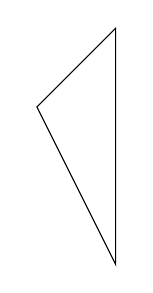
\begin{tikzpicture}
    \draw (0,0) node[anchor=north]{}
    -- (1,1) node[anchor=north]{}
    -- (1,-2) node[anchor=south]{}
    -- cycle;
  \end{tikzpicture}
  \]
  \[ S_2=\big\{(x,y): 0\leq x\leq 1, -2x\leq y\leq x\big\} \]
  Let's focus on $S=\big\{(x,y): a\leq x\leq b, \phii(x)\leq y \leq\Psi(x)\big\}$ \\
  Let's assume $f\rightarrow\BR$ is continuous. \\
\subsection*{Theorem}
  We have: \\
  \[ \iint_Sf(x,y)\,dx\,dy=\iint_Q\widetilde{f}(x,y)\,dx\,dy=\int_a^b\bigg(\int_{\phii(x)}^{\Psi(x)}f(x,y)\,dy\bigg)\,dx \]
  \begin{proof}
    Just need to go from second to third term \\
    \[ \iint_Q\widetilde{f}(x,y)\,dx\,dy=\int_a^b\bigg(\int_c^d\widetilde{f}(x,y)\,dy\bigg)\,dx=\int_a^b\bigg(\int_{\phii(x)}^{\Psi(x)}f(x,y)\,dy\bigg)\,dx \]
  \end{proof}
  The other kind of simple domains is : \\
  \[ T=\big\{(x,y)\in\BR^2:c\leq y\leq d, g(y)\leq x\leq h(y)\bigg\} \]
  for $g,h$ are continuous functions: $[c,d]\rightarrow\BR$ \\
  Same constructions as earlier \\
  Then, for $f:T\rightarrow\BR$ continuous, then \\
  \[ \iint_Tf(x,y)\,dx\,dy=\int_c^d\bigg(\int_{g(y)}^{h(y)}f(x,y)\,dx\bigg)\,dy \]
\subsection*{Remarks}
  \circled{1} Sometimes, $S$ is simple both ways \\
  Ex: $S=\overline{B}(0,1)=\big\{(x,y):x^2+y^2\leq 1\big\}$
  \begin{align*}
    S & = \big\{(x,y):-1\leq x\leq 1,-\sqrt{1-x^2}\leq y\leq\sqrt{1-x^2}\big\} \\
    & = \big\{(x,y): -1\leq y\leq 1,-\sqrt{1-y^2}\leq x\leq\sqrt{1-y^2}\big\}
  \end{align*}
  \circled{2} A complicated domain can be divided into simple domains
\subsection*{Two simple applications}
  \[ S=\big\{(x,y): a\leq x\leq b, \phii(x)\leq y\leq\Psi(x)\big\} \]
  \underline{Area of $S$} \\
  \begin{align*}
    |S| & =\text{Area of $S$}=\iint_S 1\,dx\,dy \\
    & = \int_a^b\bigg(\int_{\phii(x)}^{\Psi(x)}1\,dy\bigg)\,dx=\int_a^b(\Psi(x)-\phii(x))\,dx
  \end{align*}
  \underline{Ex}:
  \[ |S|=\int_0^1(x^2-(-x^3))\,dx=\int_0^1(x^2+x^3)\,dx=\frac{1}{3}+\frac{1}{4}=\frac{7}{12} \]
  \[ D = \big\{(x,y,z)\in\BR^3:(x,y)\in S, 0\leq z\leq f(x,y)\big\} \]
  Volume of $D$ = $|D|$ = $\iint_Sf(x,y)\,dx\,dy$
\end{document}
